%!TEX encoding = UTF-8 Unicode
%!TEX TS-program = pdflatex
\documentclass[a4paper,italian]{article}
\usepackage{lmodern}

\usepackage{amsmath,amssymb}
\usepackage{mathtools, nccmath}
\usepackage{makeidx}
\usepackage{graphicx}
%\usepackage{indentfirst}
\usepackage[parfill]{parskip}	%toglie tutte indentazioni dei paragrafi
\usepackage{paralist}
\usepackage{mathrsfs}
\usepackage{hyperref} %link cliccabili nell'indice

\usepackage{pdfpages}
\usepackage{adjustbox}
\usepackage{makecell, multirow,tabularx}  

\usepackage{shellesc}
\usepackage{minted}


\usepackage{titlesec}
\usepackage[utf8]{inputenc}
\usepackage[italian]{babel}
\usepackage[bottom]{footmisc}
\pagestyle{headings}

\begin{document}
\pagenumbering{gobble}
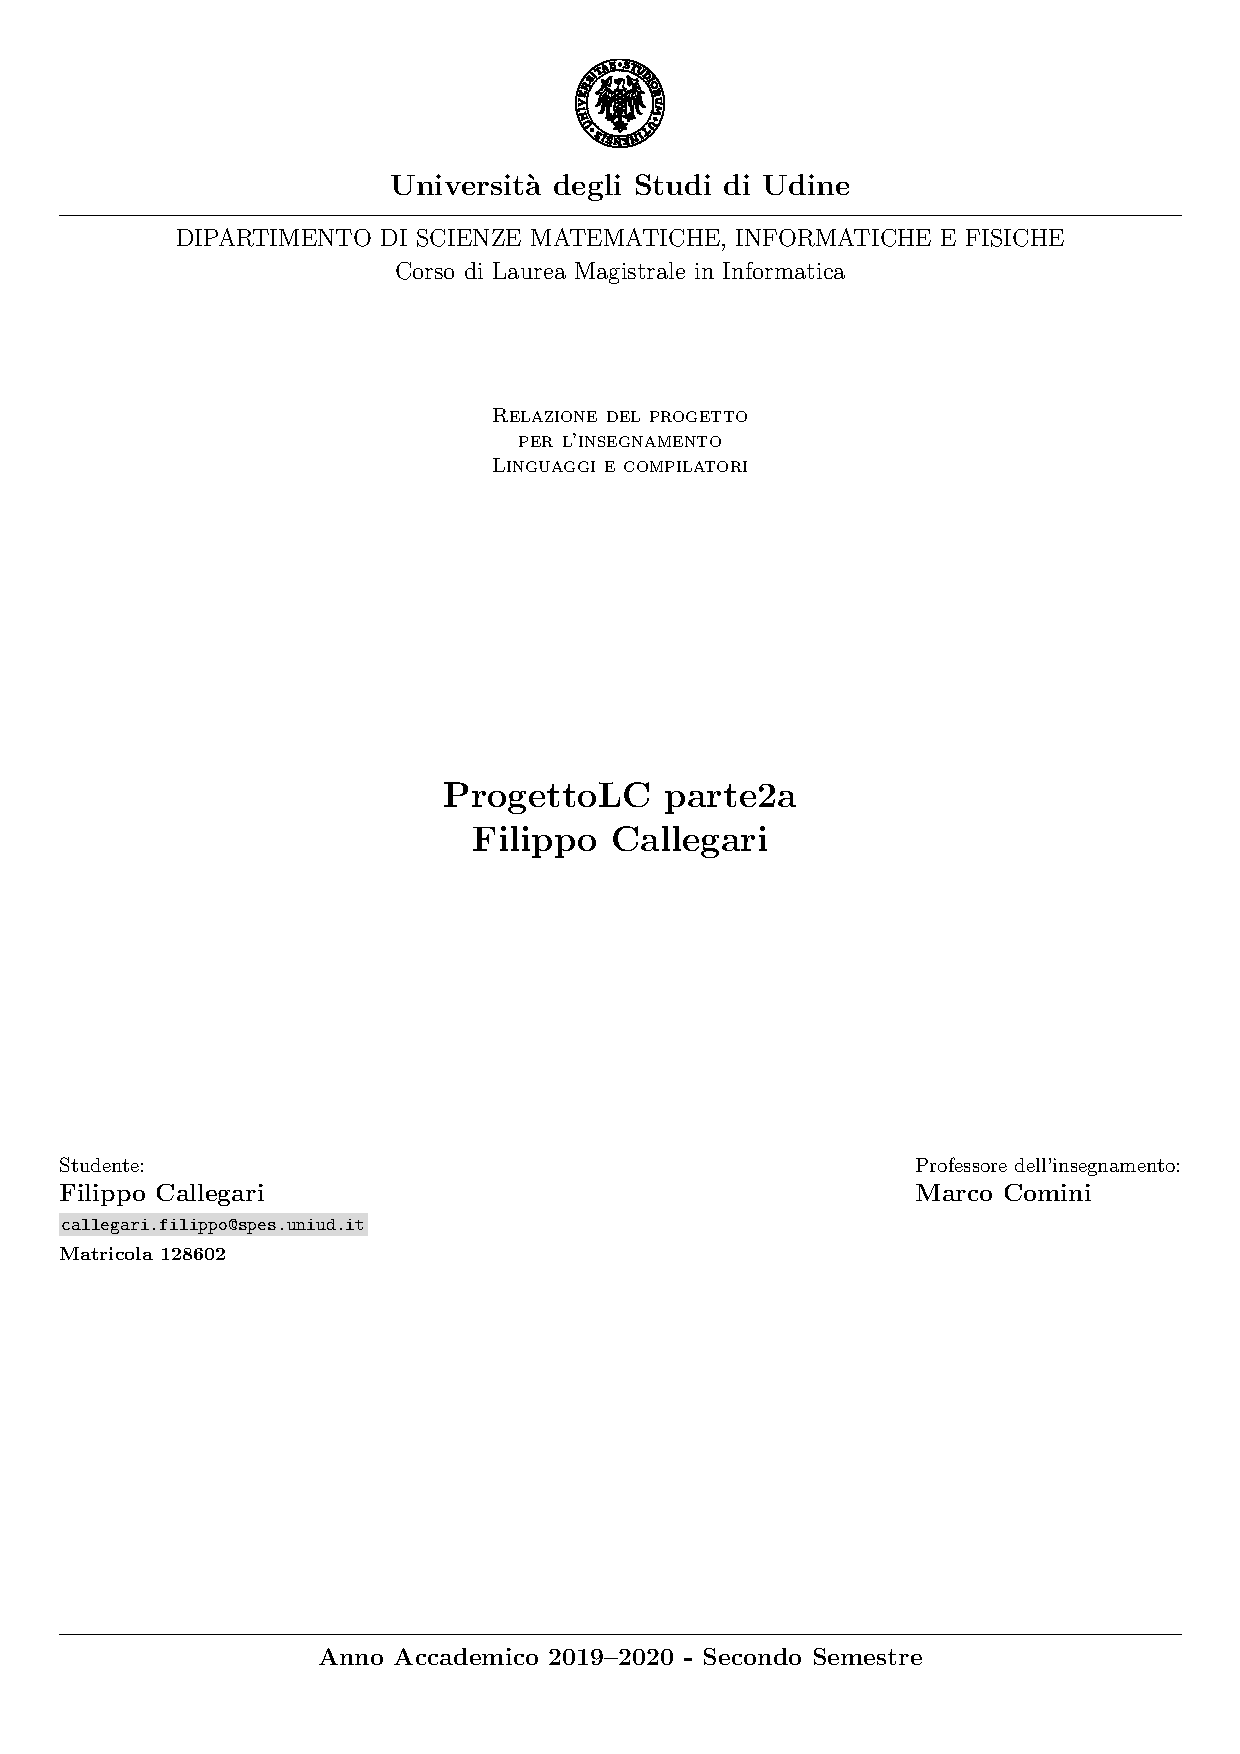
\includepdf[pages={1}]{secondafronte-frn.pdf}
\pagenumbering{arabic}
\setcounter{page}{1}

\section*{Problema e descrizione della soluzione}
Data la struttura \textit{QuadTrees}, definita come:

\begin{minted}{haskell}
  data QT a = C a 
            | Q (QT a) (QT a) (QT a) (QT a)
       deriving (Show, Eq)
\end{minted}

Dato un \texttt{QT t}, si richiede che questo abbia un \textit{bound}: ogni \texttt{t} ha un colore \texttt{C :: Integer} (sia assunto che il colore sia intero), questo deve rientrare tra un $c_{min}$ e un $c_{max}$ scelti dall'utilizzatore della funzione.

Il ``bound'' viene definito dalla funzione \texttt{bound}:
\begin{minted}{haskell}
	bound :: Ord a => a -> a -> a -> a
	bound cm cM a 
            | a > cM = cM
            | a < cm = cm
            | otherwise = a
\end{minted}
dove \texttt{cm} e \texttt{cM} sono rispettivamente $c_{min}$ e $c_{max}$ ed \texttt{a} è il ``colore''.

La soluzione proposta si avvale di \texttt{Functor} per utilizzare \texttt{fmap}, al fine di non dover definire una funzione ``mapQT'' per manipolare (e involontariamente \textit{``unwrappare''}) \texttt{QT t}.

Tale funzione sarebbe definita similmente a:
\begin{minted}{haskell}
    mapQT :: (a -> b) -> QT a -> QT b
    mapQT f (C x) = C $ f x
    mapQT f (Q ss sd is id) = Q (mapQT f ss) (mapQT f sd)
                                (mapQT f is) (mapQT f id)
\end{minted}

Viene quindi sostituita dall'istanziazione automatica per il \texttt{Functor} come segue:
\begin{minted}{haskell}
    instance Functor QT where
      fmap f (C x) = C $ f x
      fmap f (Q ss sd is id) = Q (fmap f ss) (fmap f sd)
                                 (fmap f is) (fmap f id)
\end{minted}
La soluzione adottata è quella di ``derivare'' \texttt{Functor} nella definizione di \texttt{QT}, provocando il medesimo effetto descritto sopra.

In questa maniera la soluzione viene data per composizione:
\begin{minted}{haskell}
  boundPicture :: Integral t => t -> t -> QT t -> QT t
  boundPicture cm cM a = (bound cm cM) <$> a
   where bound cm cM a 
            | a > cM = cM
            | a < cm = cm
            | otherwise = a
\end{minted}

Il risultato quindi è una applicazione della ``map'' ad un caso non più specifico come per le liste
ma applicato ad un tipo di dato ricorsivo. L'istanziazione del funtore permette quindi di ``istruire'' \texttt{Prelude} su come manipolare il dato per \texttt{fmap} (o, in questo caso, \texttt{<\$>}).

\section*{Assunzioni}
Viene assunto che il \texttt{QT t} rispetti le caratteristiche:
\begin{enumerate}
	\item chi passa alla funzione \texttt{boundPicture} passi un albero QT che rispetti le regole richieste;
	\item che \texttt{Color} sia per l'appunto di tipo \texttt{Integer}.
\end{enumerate}
L'unica assunzione che non porta a particolari problemi di esecuzione è che \texttt{t} non rispetti la ``forma normale'' per \texttt{QT}.

\section*{Test}
Si possono trovare alcuni test esemplificativi nel file \texttt{test.hs}.

\section*{Soluzione}
La soluzione si può trovare all'interno del file \texttt{esercizio.hs}.

\section*{Ambiente di lavoro}
Il sorgente viene quindi eseguito in ambiente con ``ghci'' alla versione 8.0.2.

\end{document}



















